

\paragraph{References.} 
The reference textbook on Gaussian processes is \citet{Rasmussen:2006aa}, \url{https://gaussianprocess.org/gpml/chapters/RW.pdf}. See also Chapter 18 on Gaussian processes of \citet{murphy2023probabilisticMLadvanced}, \url{https://probml.github.io/pml-book/book2.html}. 
For a comprehensive treatment of Gaussian processes seen as priors, we refer to Chapter 11 and Appendix I of \citet{ghosal2017fundamentals}. 
For more recent methods, we shall refer to papers.
For demos, see the scikit-learn page on Gaussian processes \url{https://scikit-learn.org/stable/modules/gaussian_process.html}.
See also the integrated nested Laplace approximation (INLA) for a related method \citep{rue2009approximate}.




%%%%%%%%%%%%%%%%%%%%%%%%%%%%%%%%%%%%%%%%%%%%%%%%%%%%%%%%%%%%%%%%%%%%%%%%%%%%%%
\section{Introduction and definitions}
%%%%%%%%%%%%%%%%%%%%%%%%%%%%%%%%%%%%%%%%%%%%%%%%%%%%%%%%%%%%%%%%%%%%%%%%%%%%%%

We start with definitions and basic properties fo Gaussian processes. 


\begin{definition}%{Gaussian process}
	A \alert{Gaussian process} is a stochastic process $W =(W_t: t \in T)$ indexed by an arbitrary set $T$ such that the vector $(W_{t_1},\ldots,W_{t_k})$ has a multivariate
normal distribution, for every $t_i\in T$ and $k\in \mathbb{N}$. A Gaussian process $W$ indexed by $\mathbb{R}^d$ is called:
\begin{itemize}
	\item  \alert{self-similar} of index $\alpha$ if $(W_{\sigma t}:t \in \mathbb{R}^d)$ is distributed like $(\sigma^\alpha W_{t}:t \in \mathbb{R}^d)$, for every $\sigma  > 0$, and 
	\item \alert{stationary} if $(W_{t+h}:t \in \mathbb{R}^d)$  has the same distribution of $(W_{t}:t \in \mathbb{R}^d)$, for every $h\in \mathbb{R}^d$.
\end{itemize}
\end{definition}



Vectors $(W_{t_1},\ldots,W_{t_k})$ are called \alert{marginals}, and their distributions \alert{marginal distributions} or \alert{finite-dimensional distributions}. Since a multivariate normal distribution is characterized by its mean vector and covariance matrix, the finite-dimensional distributions are determined by the \alert{mean function} and \alert{covariance kernel}, defined by
$$\mu(t) = \mathbb{E}(W_t), \quad 
K(s, t) = \text{Cov}(W_s, W_t), \quad s, t \in  T.$$

If $W =(W_t: t \in \mathbb{R}^d)$ is a Gaussian process  with covariance kernel $K$, then the process $(W_{\sigma t}: t \in \mathbb{R}^d)$ is another Gaussian process, with covariance kernel $K(\sigma s, \sigma t)$, for any $\sigma  > 0$. A scaling factor $\sigma  > 1$ shrinks the sample paths, whereas a factor $\sigma  < 1$ stretches them.

\begin{center}
	$\sigma  > 1$ \hspace{4.5cm} $\sigma  < 1$ 
	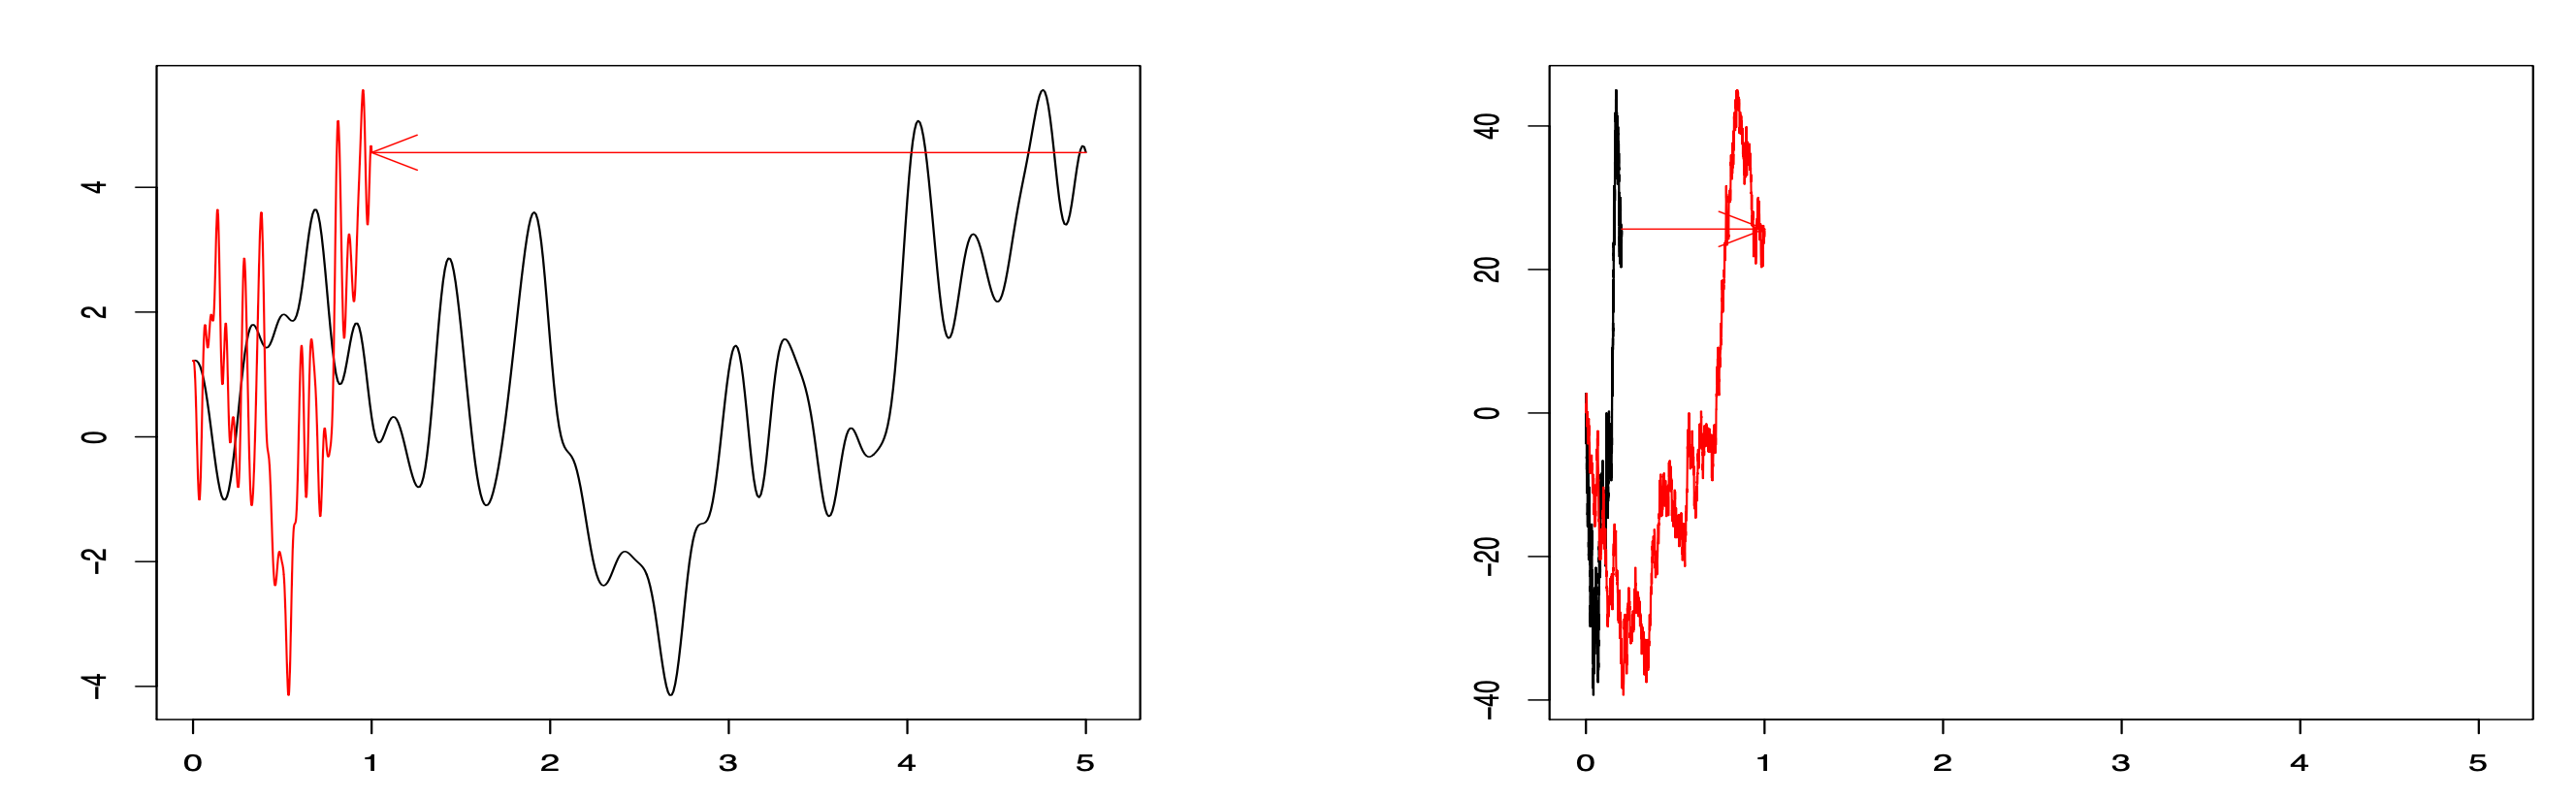
\includegraphics[width=.9\textwidth]{figures_julyan/gp/scaling}
\end{center}
\hfill From \citet{ghosal2017fundamentals}

%%%%%%%%%%%%%%%%%%%%%%%%%%%%%%%%%%%%%%%%%%%%%%%%%%%%%%%%%%%%%%%%%%%%%%%%%%%%%%
\section{Examples of Gaussian processes}
%%%%%%%%%%%%%%%%%%%%%%%%%%%%%%%%%%%%%%%%%%%%%%%%%%%%%%%%%%%%%%%%%%%%%%%%%%%%%%


\begin{example}\textbf{Random series.}
	If $Z_1,\ldots,Z_m\simiid \mathcal{N}(0,1)$ and $a_1,\ldots,a_m$ are [deterministic] functions, then the \textit{Random series} $W_t = \sum_{i=1}^m a_i(t)Z_i$ defines a Gaussian process with $\mu(t)=0$ and $K(s, t)= \sum_{i=1}^m a_i(t)a_i(s)$.
\end{example}






\begin{exampleT}\textbf{Brownian motion (or Wiener process).}
	The \textit{Brownian motion} is the zero-mean Gaussian process, say on $[0,\infty)$, with continuous sample paths and covariance function $K(s,t)=\min(s,t)$.
\end{exampleT}



	Let $B_t$ be a Brownian motion. It is:
	\begin{itemize}
		\item \alert{Stationarity}:  $\forall s< t$, $B_t-B_s\sim \mathcal{N}(0,t-s)$.
		\item \alert{Independent increments}:  $\forall s< t$, $(B_t-B_s)\indep (B_u, u\leq s)$.
	\end{itemize}
	Thus it is a L\'evy process (a stochastic process with independent, stationary increments).
	\begin{itemize}
		\item \alert{Self-similar} of index $1/2$.
	\end{itemize}






\begin{example}\textbf{Ornstein--Uhlenbeck.}
	The standard \textit{Ornstein--Uhlenbeck process} with parameter $\theta>0$ is a mean-zero, stationary GP with time set $T = [0, \infty)$, continuous sample paths, and covariance function
		$$K(s,t) = (2\theta)^{-1}\exp\left(-\theta|t-s|\right).$$
\end{example}

	The standard Ornstein--Uhlenbeck process with parameter $\theta>0$ can be constructed from a Brownian motion $B$ through the relation 	
	$$W_t = (2\theta)^{-1/2}\exp\left(-\theta t\right)B_{e^{2\theta t}}.$$

\citet{mandt2017stochastic} describes a relationship between [fixed learning rate] \alert{stochastic gradient descent} (SGD) and \alert{Markov chain Monte Carlo} (MCMC) through the Ornstein--Uhlenbeck process.







	
\begin{example}\textbf{Square exponential.}
	GP with covariance function (a.k.a. radial basis function kernel)
	$$K(s,t) = \exp\left(-\frac{\Vert t-s\Vert^2}{2\ell^2}\right).$$
	Parameter $\ell$ is called the \textit{characteristic length-scale}.
\end{example}


\begin{example}\textbf{Fractional Brownian motion.}
	The \textit{fractional Brownian motion} (fBm) with \textit{Hurst parameter} $\alpha\in  (0, 1)$ is the mean zero Gaussian process $ W = (W_t : t \in  [0, 1])$ with continuous sample paths and covariance function
	$$K(s,t) = \frac{1}{2}\left(s^{2\alpha}+t^{2\alpha}-|t-s|^{2\alpha}\right).$$
	\begin{itemize}
		\item $\alpha=2$ yields the standard Brownian motion.
	\end{itemize}
\end{example}
	





\begin{example}\textbf{Kriging.}
	For a given Gaussian process $W = (W_t : t \in T)$ and fixed, distinct points $t_1,\ldots,t_m \in T$, the conditional expectations $W_t^\star  = \mathbb{E}[ W_t|W_{t_1},\ldots,W_{t_m}]$ define another Gaussian process.
\end{example}


Properties of Kriging:
	\begin{itemize}
		\item If $W$ has continuous sample paths, then so does $W^\star$. 
		\item In that case the process $W^\star$ converges to $W$ when $m \to \infty$  and the interpolating points $(t_1,\ldots,t_m)$ grow dense in $T$.
	\end{itemize}
	
	
%%%%%%%%%%%%%%%%%%%%%%%%%%%%%%%%%%%%%%%%%%%%%%%%%%%%%%%%%%%%%%%%%%%%%%%%%%%%%%
\section{Reproducing kernel Hilbert space}
%%%%%%%%%%%%%%%%%%%%%%%%%%%%%%%%%%%%%%%%%%%%%%%%%%%%%%%%%%%%%%%%%%%%%%%%%%%%%%


	To every Gaussian process corresponds a Hilbert space, determined by its covariance kernel. This space determines the support and shape of the process, and therefore is crucial for the properties of the Gaussian process as a prior. 


\begin{definition}
	A \textit{Hilbert space} is an inner product space that is complete wrt the distance function induced by the inner product.
\end{definition}



For a Gaussian process $W = (W_t : t \in T)$, let $\overline{\text{lin}}(W)$ be the closure of the set of all linear combinations $\sum_I \alpha_i W_{t_i}$ in the $L_2$-space of square-integrable variables. The space $\overline{\text{lin}}(W)$ is a Hilbert space.

\begin{definition} 
The \textit{reproducing kernel Hilbert space} (RKHS) of the mean-zero, Gaussian process $W = (W_t : t \in T )$ is the set $\mathbb{H}$ of all functions $z_H:T \to \mathbb{R}$ defined by $z_H(t) = \mathbb{E}(W_t H)$, for $H$ ranging over $\overline{\text{lin}}(W)$. The corresponding inner product is
	$$\langle z_{H_1},z_{H_2}\rangle_{\mathbb{H}} =  \mathbb{E}(H_1H_2).$$
\end{definition}


The reproducing kernel Hilbert space has the following properties:
	\begin{itemize}
		\item Correspondance $z_H \leftrightarrow H$ is an isometry (by def of inner product), so the definition is well-posed (the correspondence is one-to-one), and $H$ is indeed a Hilbert space.
		\item Function corresponding to $H=\sum_I \alpha_i W_{s_i}$ is \bigskip
			$z_H=$
		\item For any $s\in T$, function $K(s,\cdot)$ is in RKHS $\mathbb{H}$ associated with $H = W_s$.
	\end{itemize}


Reproducing formula:
For a general function $z_H \in \mathbb{H}$ we have $$\langle z_H, K(s, \cdot)\rangle_{\mathbb{H}} = \mathbb{E}(H W_s) = z_H(s).$$
That is to say, for any function  $h \in \mathbb{H}$,
	$$h(t) = \langle h, K(t, \cdot)\rangle_{\mathbb{H}}.$$




%\begin{frame}{Example of RKHS: Euclidean space}
%	\begin{example}{Euclidean space}
%		
%	\end{example}
%	\vfill 


